\chapter{IPv6-SLAAC}
\label{chap:ipv6_slaac}

\section{Ejercicio 2.1}
\subsection{Muestra una captura del escenario en el momento inicial de la simulación en la que se vean todas las
direcciones MAC e IP. Utilizando la dirección IP de host[0] como ejemplo, explica cómo se construye, destacando
los campos y bits relevantes. Utiliza para explicarlo la notación IPv6 no abreviada (16 bytes:
xxxx:xxxx:xxxx:xxxx:xxxx:xxxx:xxxx:xxxx)}

\begin{figure}[!ht]
    \centering
    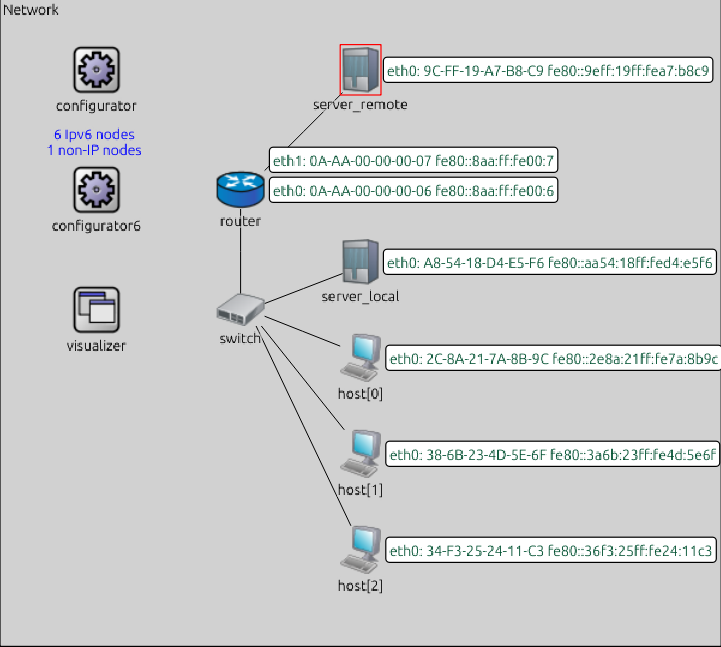
\includegraphics[width=135mm, scale=0.75]{imaxes/captura_ejer2_1.png}
    \caption{Escenario inicial dispositivos con IPv6}
    \label{fig:direccion_ipv6_host0}
\end{figure}

En el principio de la simulación, la direcciones que se muestran son direcciones unicast local de enlace. Estas son direcciones se generan automáticamente una vez que un dispositivo se conecta a una red. La estructura de este tipo de direcciones tienen como prefijo FE80::, no se enrutan y son únicas en ese enlace específico.

La segunda parte de la dirección se forma a partir de la dirección MAC del dispositivo. Para esto, fijamos el séptimo bit a 1 e insertamos 0XFFFE entre las dos mitades de la dirección MAC del dispositivo. 

Como ejemplo, vamos a ver la dirección unicast local de enlace que genera el dispositivo host[0]. Como vemos en la imagen \ref{fig:direccion_ipv6_host0}, su dirección está formada como primera parte FE80:: y la segunda parte como 2E8A:21FF:FE7A:8B9C. Esa segunda parte, como se explicó antes, se forma a partir de su dirección MAC (2C-8A-21-7A-8B-9C). Como vemos, en los primeros 2 bytes de la dirección unicast local de enlace (2E8A), si lo comparamos con su dirección MAC, pasa a ser la segunda una E ya que tenemos que añadir un uno en el séptimo bit (la letra C hexadecimal, en binario es 1100, como su tercer bit corresponde al séptimo bit de la dirección unicast, pasa a ser 1 por lo que se convirte en E -> 1110). Llegados a este punto y al haber hecho el primer cambio, tenemos la siguinte estructura -> FE80::2E80:21

Como se explicó anteriormente, una vez hecho el primer cambio, ahora añadimos 0XFFFE  y posteriormente los últimos 3 bytes de la dirección MAC, por lo que queda como dirección final unicast local de enlace FE80::2E8A:21FF:FE7A:8B9C


\section{Ejercicio 2.2}\label{chap:ejer22}
\subsection{Asigna al host[2] la misma dirección MAC que al host[0] y arranca la simulación. ¿Qué error ocurre antes de
que haya transcurrido el primer segundo de simulación? Muestra una captura del error que aparece. ¿Qué
paquete (tipo, origen y destino) provoca el error? ¿Por qué?}

\begin{figure}[!ht]
    \centering
    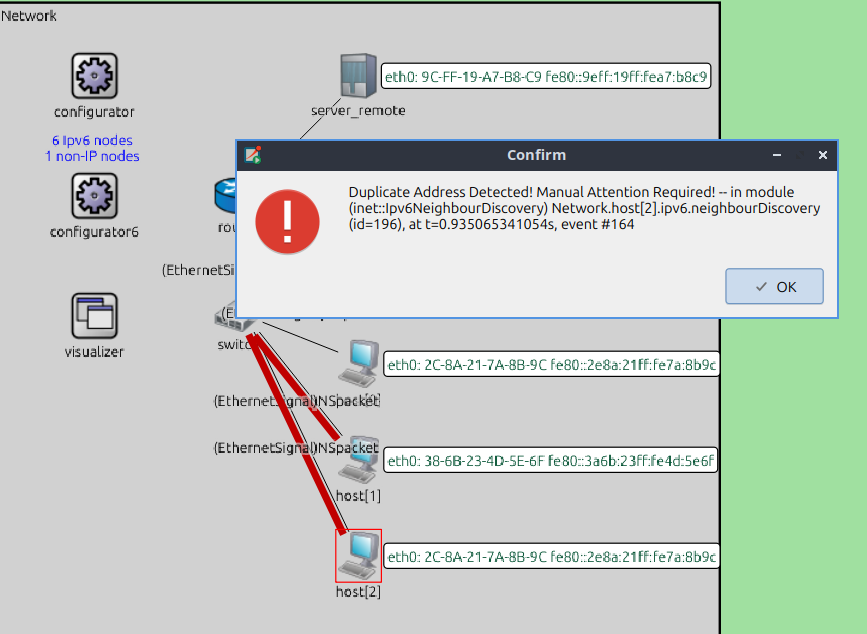
\includegraphics[width=135mm, scale=0.75]{imaxes/captura_ejer2_2.png}
    \caption{Fallo en la red con MAC host[2] igual a la de host[0]}
    \label{fig:fallo_ipv6_host2}
\end{figure}

Tal y como se muestra en la imagen \ref{fig:fallo_ipv6_host2}, hay un fallo de direcciones duplicadas cuando el host[2] intenta asignarse una dirección IPv6. 

El paquete en concreto que provoca el error es de tipo ICMPv6 con mensaje NS (Neighbor Solicitation), donde el origen de momento es el host[2] (en ese momento sin ninguna dirección) y como destino una dirección multicast. Este error ocurre porque el host[2], cuando crea su dirección, le comunica a sus vecinos de la red (DAD) como es su dirección entonces se encuentra que el host[0] tiene la misma dirección IPv6 que el se asigno por lo que ocurre un conflito de IPs.

\section{Ejercicio 2.3}
\subsection{Cambia la MAC del host[2] de manera que coincida con la de host[0] en los últimos 3 bytes y difiera en los 3
primeros bytes (mantén esta MAC para el resto de las cuestiones). Asigna a serverremote la misma MAC que a
host[0]. ¿Vuelve a ocurrir el error de dirección duplicada con serverremote y host[0]? ¿Por qué?}

En este caso, al poner la misma MAC al host[0] y al server remote no produce ningún error porque son dispositivos que están en diferentes redes. 
El conflito que sucedía en el ejercicio \ref{chap:ejer22} es porque los dos dispositivos estaban en la misma red por lo que salta el error de 
direcciones duplicadas. Esto es como en IPv4 con las IPs privadas, en la misma red no puede haber dos IPs iguales pero si hay dos redes diferentes, puede coincidir una IP privada de un dispositivo que está en la red1 con otra IP privada de otro dispositivo que está en la red2

\section{Ejercicio 2.4}
\subsection{¿Cuánto tiempo transcurre desde el principio de la simulación hasta que el host[0] su IP link-local definitiva
(i.e., fin de DAD)? Muestra la tabla de interfaces del nodo host[0] en la que se vea su estado antes y después del
DAD timeout y explica qué cambia. (Nota: Qtenv muestra toda la información de cada interfaz en una línea;
para verla correctamente copia el contenido con botón derecho → Copy Value y pégalo en la memoria como
texto, en lugar de usar capturas de pantalla.)}

\section{Ejercicio 2.5}
\subsection{¿En qué instante de la simulación obtienen los equipos sus direcciones IP globales? ¿Cómo obtienen esta
última? Muestra la tabla de interfaces de nodo host[0] en la que se vea su estado antes y después de obtener la
dirección global y explica qué cambia.}

\section{Ejercicio 2.6}
\subsection{Explica cómo se construye la IP global usando el nodo host[0] como ejemplo, de nuevo usando la notación
IPv6 no abreviada}

Una vez que el equipo manda un mensaje ICMPv6 con mensaje NS (Neighbor Solicitation) y no ocurre ningún fallo (no hay conflicto de IPs), procede a mandar un paquete ICMPv6 con mensaje RS (Router Solicitation), para que el router le asigne unha IPv6 global (este tipo de IPs ya son enrrutables y únicas a nivel global). El router contesta con un paquete ICMPv6 con mensaje RA (Router Advertisement) indicando el prefijo global de red (los primeros 64 bits de la dirección de la red al que está conectada host[0], en este caso AAAA:0006:0065:0000). Una vez que el host[0] obtiene el prefijo de la red, construye su IPv6 global substituyendo el prefijo de red del enlace local por la de la red quedando su dirección como: AAAA:0006:0065:0000:2E8A:21FF:FE7A:8B9C. Esto se puede ver en la imagen \ref{fig:ip_global_host0}

\begin{figure}[H]
    \centering
    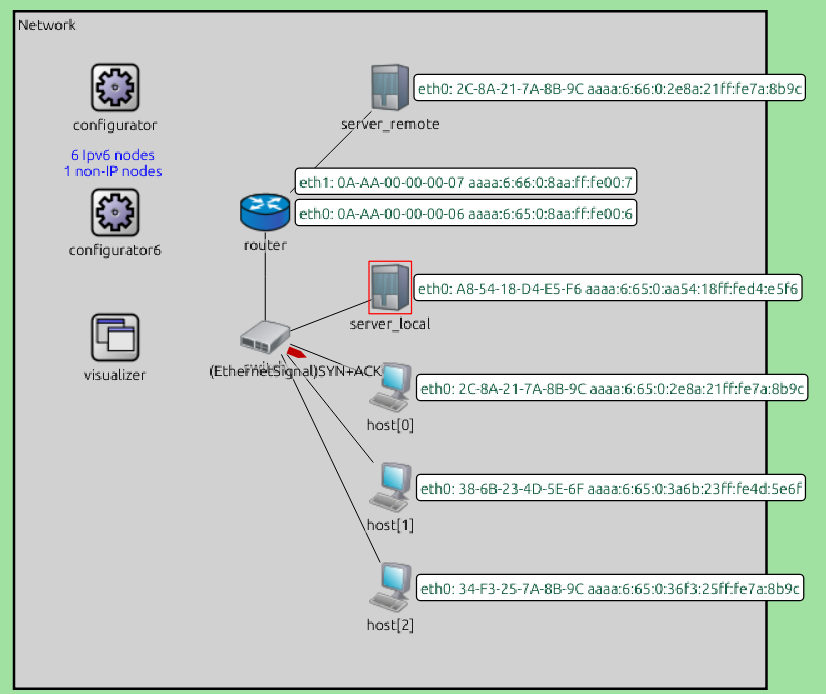
\includegraphics[width=135mm, scale=0.75]{imaxes/captura_ejer2_6.png}
    \caption{Foto red con direcciones IPv6 globales asignadas}
    \label{fig:ip_global_host0}
\end{figure}

\section{Ejercicio 2.7}
\subsection{Configura host[0] para que se conecte al servidor server remote usando su dirección fe80::x:x:x:x:
(asegúrate de que la dirección MAC de server remote es única). ¿Qué ocurre? Repite lo mismo para
server local. ¿Qué ocurre?}